\documentclass[a4paper,10pt,oneside]{article}
\usepackage{graphicx}
\usepackage{color}
\usepackage{url}
\usepackage{subfigure}
\usepackage[utf8]{inputenc}
\usepackage[T1]{fontenc}
\usepackage{tgpagella}
%\usepackage[scale=0.9]{tgcursor}
%\usepackage[scale=0.9]{tgheros}
\usepackage{xstring}

\newcommand{\myscale}{0.74}
\newcommand{\vect}[1]{\boldsymbol{#1}}
\newcommand{\code}[1]{\texttt{\StrSubstitute{#1}{.}{.\.}}}
\def\.{\discretionary{}{}{}}
\newcommand{\jmodule}[1]{\texttt{\textit{#1}}}

\setlength{\hoffset}{-1in} %left margin will be 0, as hoffset is by default 1inch
\setlength{\voffset}{-1in} %analogous voffset
\setlength{\oddsidemargin}{1.5cm}
\setlength{\evensidemargin}{1.5cm}
\setlength{\topmargin}{1.5cm}
\setlength{\textheight}{24cm}
\setlength{\textwidth}{18cm}

\def\mftitle{jInfer TreeRuleDisplayer Module Description}
\def\mfauthor{Michal Klempa, Mário Mikula, Robert Smetana, Michal Švirec, Matej Vitásek}
\def\mfadvisor{RNDr. Irena Mlýnková, Ph.D., Martin Nečaský, Ph.D.}
\def\mfplacedate{Praha, 2011}
\title{\bf\mftitle}
\author{\mfauthor \\ Advisors: \mfadvisor}
\date{\mfplacedate}

\ifx\pdfoutput\undefined\relax\else\pdfinfo{ /Title (\mftitle) /Author (\mfauthor) /Creator (PDFLaTeX) } \fi

\begin{document}
\maketitle
\noindent Target audience: developers willing to extend jInfer, looking for ways to visualize grammars.

\noindent \begin{tabular}{|l|l|} \hline
Responsible developer & Michal Švirec \\ \hline
Required tokens       & none \\ \hline
Provided tokens       & \code{cz.cuni.mff.ksi.jinfer.base.interfaces.RuleDisplayer} \\ \hline
Module dependencies   & Base \\
	& JUNG \\ \hline
Public packages       & none \\ \hline
\end{tabular}

\section{Introduction}

This rule displayer uses JUNG graph implementation to draw rules as a forest of trees, where each tree represents one rule from the whole set. In each tree, root vertex represents left side of the rule, inner vertices represents concatenation, alternation or permutation and leafs are elements, simple data or attribute. As in basic rule displayer, tree rule displayer creates a component with multiple tabs: each one for a new grammar to display.

\section{Structure}

The main class implementing \code{RuleDisplayer} inference interface and simultaneously being registered as its service provider is \code{TreeRuleDisplayer}. Main method of this class is \code{createDisplayer()}, which looks up the component, adds a new panel to it, and renders the specified grammar in it.\\

\begin{figure}
	\centering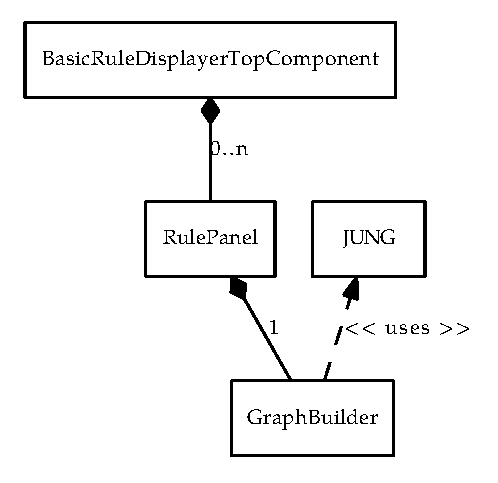
\includegraphics[scale=\myscale]{class-diagram}
	\caption{TreeRuleDisplayer class diagram} \label{figure-class-diagram}
\end{figure}

The diagram of classes involved in the process of rule displaying is in figure \ref{figure-class-diagram}. Main window of rule displayer may have multiple tabs in it: each contains its own \code{RuleDisplayer} responsible for rendering specified grammar using \jmodule{JUNG} library. Each tab in rule displayer window is represented by instance of \code{RulePanel} which contains button linking to options and the main panel (canvas) with rendered rules. Canvas is created by \code{VisualizationViewer} instance with \code{TreeLayout} layout (which are both classes from JUNG library). For \code{VisualizationViewer}, \code{GraphMouse} is set with transforming mode to allows zooming and moving of graph in canvas. To allow the user to set custom appearance of rules, we set various \code{Transformer}s in \code{RenderContext} of \code{VisualizationViewer}. These transormers change color, shape and vertex size in each rule tree according to properties set in options.\\

All the trees representing rules are created in the \code{GraphBuilder} class using the \code{buildGraphPanel()} method. This method creates \code{DelegateForrest} of \code{DelegateTree}s where each tree of the forest represents one rule. Each vertex of the tree is represented by \code{Regexp<?\ extends AbstractNamedNode>} and edge by \code{RegexpInterval}. While the code building tree structure is a nice recursion programming exercise, there is nothing of a special interest in it. Finally, the method appends forrest into layout and \code{VisualizationViewer} which were described above. All the code responsible for building rule trees is contained in the \code{cz.cuni.mff.ksi.jinfer.treeruledisplayer.logic}. For more details about JUNG library please see \cite{jung}.\\

All graphics used by \jmodule{TreeRuleDisplayer} is contained in the \code{cz.cuni.mff.ksi.jinfer.treeruledisplayer.graphics} package.

\subsection{Settings}

All settings provided by \jmodule{TreeRuleDisplayer} are NetBeans-wide. The options panel along with all the logic is in \code{cz.cuni.mff.ksi.jinfer.treeruledisplayer.options} package. Available options include setting the color of the background, horizontal and vertical distance between vertices. Also, for each type of vertex, it is possible to set a size, shape and a color.

\nocite{*}
\newpage
\bibliographystyle{alpha}
\bibliography{literature}

\end{document}
